%package list
\documentclass{article}
\usepackage[top=3cm, bottom=3cm, outer=3cm, inner=3cm]{geometry}
\usepackage{graphicx}
\usepackage{url}
%\usepackage{cite}
\usepackage{hyperref}
\usepackage{array}
%\usepackage{multicol}
\newcolumntype{x}[1]{>{\centering\arraybackslash\hspace{0pt}}p{#1}}
\usepackage{natbib}
\usepackage{pdfpages}
\usepackage{multirow}
\usepackage{multirow}
\usepackage[normalem]{ulem}
\usepackage{svg}
\usepackage{xcolor}
\usepackage{listings}
\lstdefinestyle{ascii-tree}{
    literate={├}{|}1 {─}{--}1 {└}{+}1 
  }
\lstset{basicstyle=\ttfamily,
  showstringspaces=false,
  commentstyle=\color{red},
  keywordstyle=\color{blue}
}
\useunder{\uline}{\ul}{}


%%%%%%%%%%%%%%%%%%%%%%%%%%%%%%%%%%%%%%%%%%%%%%%%%%%%%%%%%%%%%%%%%%%%%%%%%%%%
%%%%%%%%%%%%%%%%%%%%%%%%%%%%%%%%%%%%%%%%%%%%%%%%%%%%%%%%%%%%%%%%%%%%%%%%%%%%
\newcommand{\csemail}{dcasass@ulasalle.edu.pe}
\newcommand{\csdocente}{MSc. Vicente Enrique Machaca Arceda}
\newcommand{\cscurso}{Teoría de la computación}
\newcommand{\csuniversidad}{Universidad La Salle}
\newcommand{\csescuela}{Escuela Profesional de Ingeniería de Software}
\newcommand{\cspracnr}{01}
\newcommand{\cstema}{Implementación de autómatas}
%%%%%%%%%%%%%%%%%%%%%%%%%%%%%%%%%%%%%%%%%%%%%%%%%%%%%%%%%%%%%%%%%%%%%%%%%%%%
%%%%%%%%%%%%%%%%%%%%%%%%%%%%%%%%%%%%%%%%%%%%%%%%%%%%%%%%%%%%%%%%%%%%%%%%%%%%


\usepackage[english,spanish]{babel}
\usepackage[utf8]{inputenc}
\AtBeginDocument{\selectlanguage{spanish}}
\renewcommand{\figurename}{Figura}
\renewcommand{\refname}{Referencias}
\renewcommand{\tablename}{Tabla} %esto no funciona cuando se usa babel
\AtBeginDocument{%
	\renewcommand\tablename{Tabla}
}

\usepackage{fancyhdr}
\pagestyle{fancy}
\fancyhf{}
\setlength{\headheight}{30pt}
\renewcommand{\headrulewidth}{1pt}
\renewcommand{\footrulewidth}{1pt}
\fancyhead[L]{\raisebox{-0.2\height}{
\includegraphics[width=1.5cm]{logo-universidad-la-salle.png}}}
\fancyhead[C]{}
\fancyhead[R]{\fontsize{7}{7}\selectfont	\csuniversidad \\ \csescuela \\ \textbf{\cscurso} }
\fancyfoot[L]{Stds. Daniel Casas - Bekam Huaracha}
\fancyfoot[C]{CT}
\fancyfoot[R]{Página \thepage}

% para el codigo fuente
\usepackage{listings}
\usepackage{color, colortbl}
\definecolor{dkgreen}{rgb}{0,0.6,0}
\definecolor{gray}{rgb}{0.5,0.5,0.5}
\definecolor{mauve}{rgb}{0.58,0,0.82}
\definecolor{codebackground}{rgb}{0.95, 0.95, 0.92}
\definecolor{tablebackground}{rgb}{0.0, 0.45, 0.63}

\lstset{frame=tb,
	language=bash,
	aboveskip=3mm,
	belowskip=3mm,
	showstringspaces=false,
	columns=flexible,
	basicstyle={\small\ttfamily},
	numbers=none,
	numberstyle=\tiny\color{gray},
	keywordstyle=\color{blue},
	commentstyle=\color{dkgreen},
	stringstyle=\color{mauve},
	breaklines=true,
	breakatwhitespace=true,
	tabsize=3,
	backgroundcolor= \color{codebackground},
}


\begin{document}
	
	\vspace*{10px}
	
	\begin{center}	
		\fontsize{17}{17} \textbf{ Práctica \cspracnr}
	\end{center}
	%\centerline{\textbf{\underline{\Large Título: Informe de revisión del estado del arte}}}
	%\vspace*{0.5cm}
	

	\begin{table}[h]
		\begin{tabular}{|x{4.7cm}|x{4.8cm}|x{4.8cm}|}
			\hline 
			\textbf{DOCENTE} & \textbf{CARRERA}  & \textbf{CURSO}   \\
			\hline 
			\csdocente & \csescuela & \cscurso    \\
			\hline 
		\end{tabular}
	\end{table}	
	
	
	\begin{table}[h]
		\begin{tabular}{|x{4.7cm}|x{4.8cm}|x{4.8cm}|}
			\hline 
			\textbf{PRÁCTICA} & \textbf{TEMA}  & \textbf{DURACIÓN}   \\
			\hline 
			\cspracnr & \cstema & 6 horas   \\
			\hline 
		\end{tabular}
	\end{table}
	
	
	\section{Datos de los estudiantes}
	\begin{itemize}
		\item Grupo: Teoría de la computación - 23
		\item Integrantes: 
		\begin{itemize}
			\item Bekam Eddy Huaracha Cabrera
			\item Daniel Antonio Casas Soto
		\end{itemize}		
	\end{itemize}
	
		
	\section{Ejercicios}\label{sec:ejercicios}
	\begin{enumerate}
		\item Implemente un programa en Python para la representación de Automatas. Este programa deberá tener las siguientes entradas:
		\begin{itemize}
			\item Archivo CSV con la representación de transiciones.
            \item Estado inicial.
            \item Estados finales F.
       \end{itemize}	

       Luego, debera generar 2000 palabras de forma aleatoria de diferente tamano, segun el alfabeto del lenguaje, e indicar cuales son aceptadas y cuales no, por el automata. Por ejemplo, esta podria ser la salida (en un archivo de texto) para un automata que reconoce palabras que terminan en 1 con "Lenguaje" = {0, 1}:

        \begin{lstlisting}[language=bash,caption={Definición del resultado esperado}][H]
        >> 00101 -> Aceptado
        >> 00110 -> No Aceptado
        >> 10101 -> Aceptado
        >> 00000 -> No Aceptado
    	\end{lstlisting}
     
        Finalmente, debera generar un archivo .dot con contenido en lenguaje Graphviz que represente de forma grafica el automata.
        
        \end{enumerate}

        \newpage
        \vspace*{2.5px}
		\section {Solución} \label{sec:solución}
		.................
		\begin{enumerate}
		    \item Trabajamos un ejemplo con el código presentado por el profesor, para poder utilizar la librería \textbf{pandas} para leer un .csv y generar de allí una matriz.

        \lstinputlisting[language=Python, numbers=left, caption ={Código base para resolución del problema}]{basis.py}

		    \item Con este código en mente trabajamos en poder resolver el problema.
            \item Continuaremos generando las entradas para evaluar si pertenecen al lenguaje del autómata. Para el ejemplo utilizaremos esta tabla de transformaciones.

                \begin{figure}[h]
                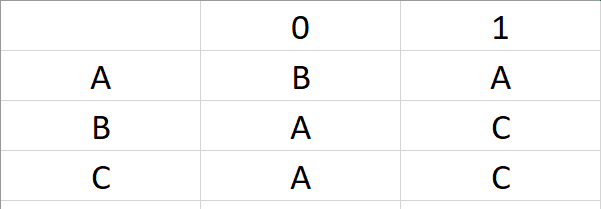
\includegraphics[width=8cm]{Tabla_csv.png}
                \end{figure}
                
            \item En base a esto podremos generar este código en Python para poder trabajar y generar los números aleatorios. Se trabajo este código: 

            \lstinputlisting[language=Python, numbers=left, caption ={Trabajo de código para construir solución}]{Primer code.py}

            Explicaremos las líneas más importantes del código que son base para el funcionamiento del problema.

            \begin{itemize}
                \item En las lineas 1-3 incluimos las importaciones de las bibliotecas necesarias: pandas para manipulación de datos tabulares, random para generar números aleatorios y sys para interactuar con la salida estándar (texto). 
                \item En las lineas 5-10 se inicializa el nombre del futuro archivo y la función 'w', que es escribir; para que se imprima en el archivo los resultados.
                \item Lineas 12-15, definimos el lenguaje y los estados de nuestro autómata.
                \item Linea 18, se inicia un bucle para iterar las 2000 palabras para el autómata.
                \item Lineas 19-22, se crea la lógica para las palabras y en cada iteración, se escriben en el documento y se almacena la palabra en 'combinación'.
                \item Lineas 24-30, se compara la locación actual en la "matriz delta" con el resultado que debería estar en esa posición, esto se hace iterando por cada dígito de la palabra.
            \end{itemize}

            Ahora nos falta poder trabajar con el código en Graphviz, con un código proporcionado por el profesor, tenemos que hacer que nuestro programa en Python devuelva una entrada como esta:

        \begin{lstlisting}[language=bash,caption={Definición del resultado esperado para Graphviz}][H]
            A -> B [label = 0 ];
            A -> A [label = 1 ];
            B -> A [label = 0 ];
            B -> C [label = 1 ];
            C -> A [label = 0 ];
            C -> C [label = 1 ];
    	\end{lstlisting}

        En base a eso, se agrego una función de un 'for' anidado que itera por cada línea de la matriz 'delta' y nos devuelve los valores de las filas y columnas, agregando a esta un valor (la locación adecuada según el autómata).

        \lstinputlisting[language=Python, numbers=left, caption ={Iterador de matriz implementado}]{SeconCode.py}

        Esta función la veremos ejemplificada en las lineas 17-23, donde recolectara el valor primero en cada fila (row) y luego en cada columna (column), para ejercerlo en el formato que hemos construido para que lo imprima. 

        \item Con esto ya resuelto, podremos ver que nos da un resultado como este: 

        \begin{lstlisting}[language=bash,caption={Definición del resultado esperado para Graphviz}][H]
            A -> B [label = 0 ];
            A -> A [label = 1 ];
            B -> A [label = 0 ];
            B -> C [label = 1 ];
            C -> A [label = 0 ];
            C -> C [label = 1 ];
            
            
            ------------------------------------------------------------
            
            
            >> 100010001111111011001011011010011  --> No Aceptado
            >> 1101100110001101010000010110010001010100000001  --> No Aceptado
            >> 101100111100  --> No Aceptado
            >> 111001100011010101101111011110100011010  --> No Aceptado
            >> 011111100111111110101000010001101000100011  --> Aceptado...
    	\end{lstlisting}

        \item Ahora procediendo a pegar la salida que nos interesa en el código .DOT para el graphviz. Tendríamos este autómata determinista.

        \begin{figure}[h]
           \centering
           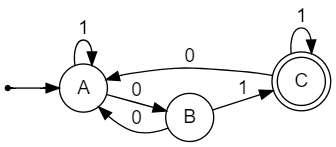
\includegraphics[width=8cm]{Auto_1.png}
        \end{figure}

        Este sería el código:

        \begin{figure}[h]
           \centering
           \includegraphics[width=8cm]{códigoDOT.png}
        \end{figure}

        \item Esto concluiría con el problema propuesto, sin embargo ahora se hace necesario poder trabajar con el desafío dado en clase:
          \begin{itemize}
              \item Probar los resultados con un autómata de 5 estados como mínimo y con este alfabeto = {0,1,2}.
          \end{itemize}

          Para trabajar con este, solamente necesitariamos determinar una matriz con estos estados y generar el código que se pidio, solamente modificando las entradas para tener el resultado esperado.

          \newpage

          Esta sería la matriz pensada:
          
          \begin{figure}[h]
           \centering
           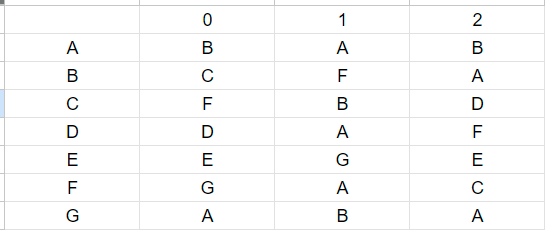
\includegraphics[width=8cm]{Tabla2.png}
        \end{figure}

        \item Modificando el código con el nuevo "alfabeto", el estado inicial nuevo "A" y los estados Finales "C" y "G". Ahora podemos general el texto para el trabajo.

        \lstinputlisting[language=Python, numbers=left, caption ={Código para autómata con 7 estados}]{Code2.py}

        Este código nos genera un archivo con los datos exactos para poder general el autómata en Graphviz, esto demostraría cual sería ese archivo.
        
        \begin{lstlisting}[language=bash,caption={Definición del resultado esperado para Graphviz v.2 (7 Estados)}][H]
            A -> B [label = 0 ];
            A -> A [label = 1 ];
            A -> B [label = 2 ];
            B -> C [label = 0 ];
            B -> F [label = 1 ];
            B -> A [label = 2 ];
            C -> F [label = 0 ];
            C -> B [label = 1 ];
            C -> D [label = 2 ];
            D -> D [label = 0 ];
            D -> A [label = 1 ];
            D -> F [label = 2 ];
            E -> E [label = 0 ];
            E -> G [label = 1 ];
            E -> E [label = 2 ];
            F -> G [label = 0 ];
            F -> A [label = 1 ];
            F -> C [label = 2 ];
            G -> A [label = 0 ];
            G -> B [label = 1 ];
            G -> A [label = 2 ];
            
            
            ------------------------------------------------------------
            
            
            >> 101122022102  --> No Aceptado
            >> 020212220001201022010211211111211000120201220  --> No Aceptado
            >> 12210221200010202210010000200000002112111211002001  --> No Aceptado
            >> 22022021022121020120022  --> No Aceptado
            >> 01210001100220202221222120102002020200  --> Aceptado  
    	\end{lstlisting} 

     \newpage

        Mostraremos cuál sería el resultado tanto en código DOT como el .png del autómata creado por la matriz.
        
         \begin{figure}[h]
           \centering
           \includegraphics[width=8cm]{códigoDOT2.png}
        \end{figure}
        \begin{figure}[h]
           \centering
           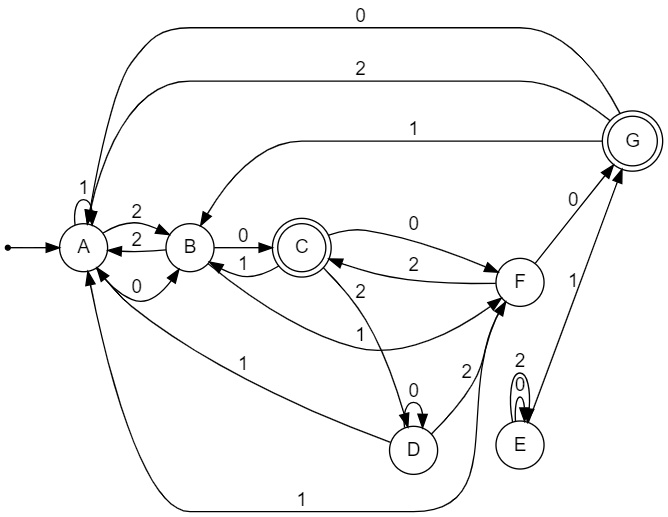
\includegraphics[width=8cm]{Auto_2.png}
        \end{figure}

        \item Se subieron los archivos y los códigos al GitHub para poder trabajar en el repositorio: CT-23 \url{https://github.com/DACS-SLL/CT-23.git}

		\end{enumerate}
	
	%\clearpage
	%\bibliographystyle{apalike}
	%\bibliographystyle{IEEEtranN}
	%\bibliography{bibliography}
		
	
\end{document}